\documentclass{hcmut-report}
\usepackage{codespace}

% Sub-preambles
% https://github.com/MartinScharrer/standalone

% Encodings
\usepackage{gensymb,textcomp}

% Better tables
% Wide tables go to https://tex.stackexchange.com/q/332902
\usepackage{array,multicol,multirow,siunitx,tabularx}

% Better enum
\usepackage{enumitem}

% Graphics
\usepackage{caption,float}
\usepackage{subcaption}

% Allow setting >max< width of figure
% 'export' allows adjustbox keys in \includegraphics
% For demonstration purposes, remove in production
\usepackage[export]{adjustbox}

% For demonstration purposes, remove in production
\usepackage{mwe}

% Configurations
\newcounter{memberrowno}
\setcounter{memberrowno}{0}

\ocoursename{AS6041 Advanced CFD}
\oreporttype{COMP SQUARE}
\title{Assignment 1}
\oadvisor{Advisor h}
\reportlayout

% Custom commands
\newcommand*\mean[1]{\bar{#1}}

\begin{document}
\coverpage

\section{Taylor green vortex simulation:}
    \subsection{turbulent kinetic energy}
    \begin{figure}[H]
        \centering
        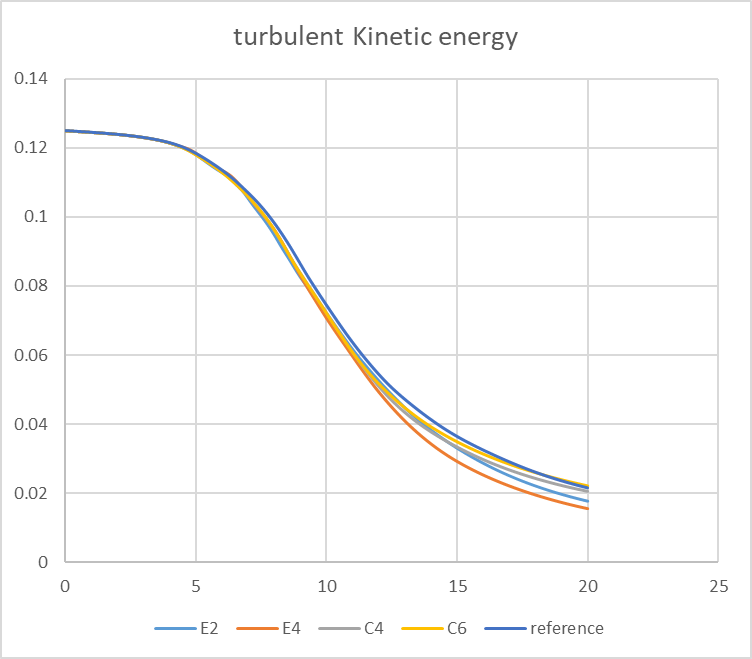
\includegraphics[width=0.45\textwidth]{graphics/tke.png}
        \caption{Turbulent kinetic energy v/s time}
        \label{fig:my_label}
    \end{figure}

    Figure 1 depicts variation of TKE with time for schemes E2,E4,C4 and C6 (all with 10th order filtering scheme with an $\alpha = 0.495$)

    We can observe that TKE decreases with time. As we are solving the the navier-stokes equations with non zero viscous terms, the eddies are being damped by viscous forces hence TKE decreases. We can also observe all the schemes resolve TKE to be somewhat lower than the reference value.

    \subsection{Enstrophy}
    \begin{figure}[H]
        \centering
        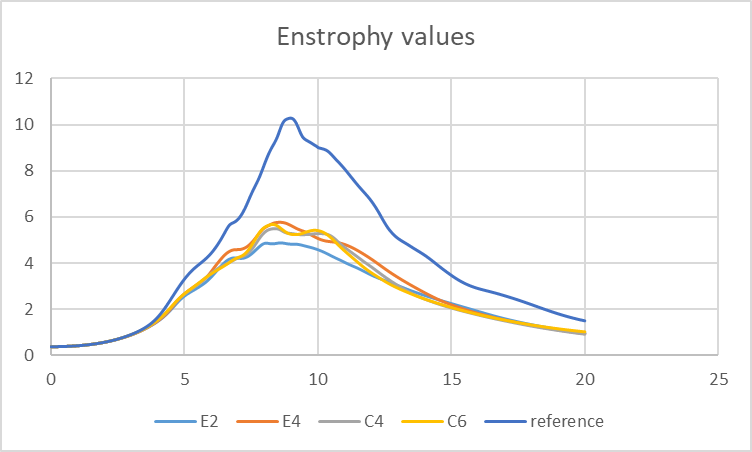
\includegraphics[width=0.6\textwidth]{graphics/enstrophy.png}
        \caption{Enstrophy vs. time}
        \label{fig:my_label}
    \end{figure}

    The enstrophy resolusion is much poorer in the case of $64\times64$ grid for all the schemes used. The resolution by E2F10 scheme is the poorest. E4F10, C4F10 and C6F10 schemes gives almost similar results.

    \subsection{Q isosurfaces}
    Shown below are the isosurface of Q criterion calculated in paraview for Q = 0.1, the colour contours on the isosurface indicates fuction 1: conservative variable 2: $\rho\times u$

    \begin{figure}[H]
     \centering
     \begin{subfigure}[b]{0.35\textwidth}
         \centering
         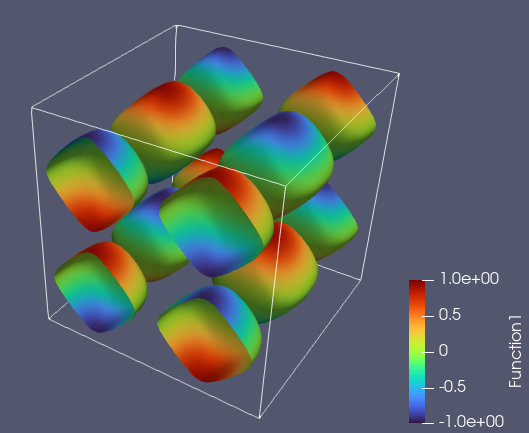
\includegraphics[width=\textwidth]{graphics/iso000.png}
         \caption{t/t$_c$ = 0}
         \label{fig:3.1}
     \end{subfigure}
     \hspace{0.5cm}
     \begin{subfigure}[b]{0.35\textwidth}
         \centering
         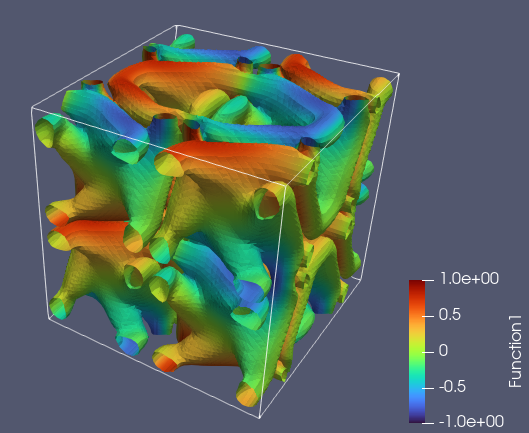
\includegraphics[width=\textwidth]{graphics/iso004.png}
         \caption{t/t$_c$ = 4}
         \label{fig:3.2}
     \end{subfigure}
     
     \begin{subfigure}[b]{0.35\textwidth}
         \centering
         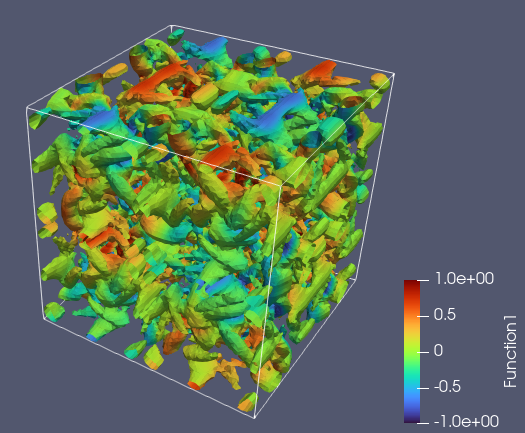
\includegraphics[width=\textwidth]{graphics/iso008.png}
         \caption{t/t$_c$ = 8}
         \label{fig:3.1}
     \end{subfigure}
     \hspace{0.5cm}
     \begin{subfigure}[b]{0.35\textwidth}
         \centering
         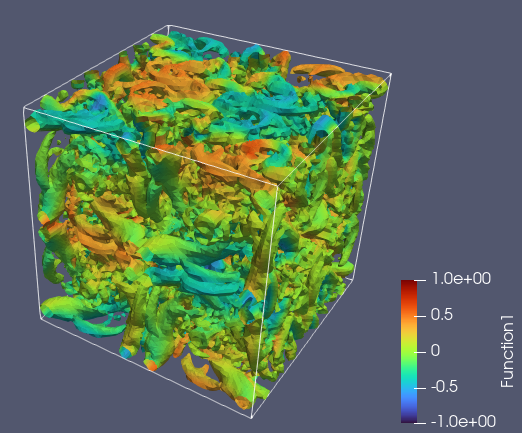
\includegraphics[width=\textwidth]{graphics/iso012.png}
         \caption{t/t$_c$ = 12}
         \label{fig:3.1}
     \end{subfigure}

     \begin{subfigure}[b]{0.35\textwidth}
         \centering
         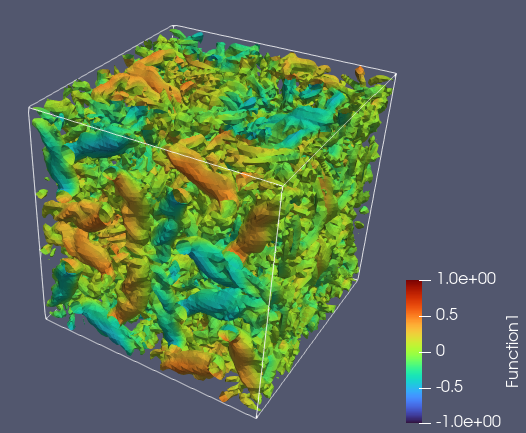
\includegraphics[width=\textwidth]{graphics/iso016.png}
         \caption{t/t$_c$ = 16}
         \label{fig:3.1}
     \end{subfigure}
     \hspace{0.5cm}
     \begin{subfigure}[b]{0.35\textwidth}
         \centering
         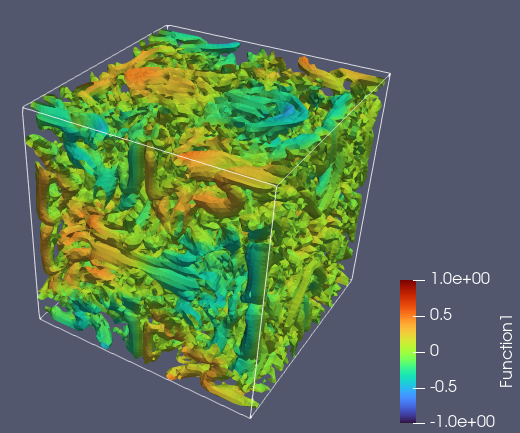
\includegraphics[width=\textwidth]{graphics/iso020.png}
         \caption{t/t$_c$ = 20}
         \label{fig:3.1}
     \end{subfigure}
     \caption{Q criterion isosurface from paraview}
     \label{fig:3}
    \end{figure}

    I calculated the velocity vector from functions 6, 7 and 8 using the calculator feature in paraview. Then used gradient option to caculate the Q criterion for the calculated velocity.

    From the above plot we can clearly see the decay of the main vortices with time.

    \subsection{Vorticity}
    \begin{figure}[h!]
        \centering
        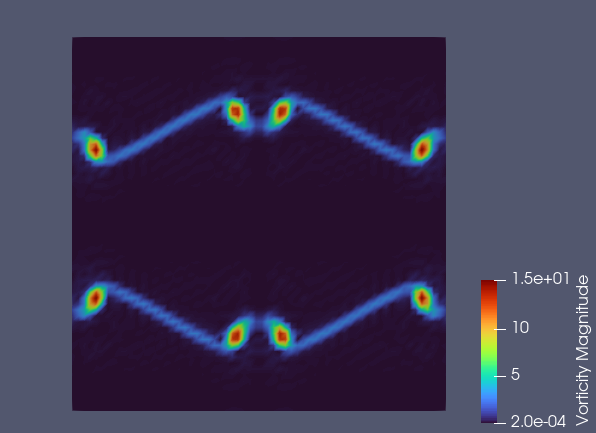
\includegraphics[width=0.5\textwidth]{graphics/vorticity.png}
        \caption{Vorticity magnitude contour}
        \label{fig:my_label}
    \end{figure}

    Calculated velocity vector from functions 6, 7 and 8. Then calculated the vorticity of the velocity field using gradient function. Then plotted contours of this vorticity magnitude on x = 3.14 slice at t/t$_c$ = 8. The figure 4 shown in reference 1 is a portion of this symmetrical vorticity contour obtained. We can see that the contour is not very well resolved. This is due to the poor element size in 64$\times$64 mesh.

    \newpage
    \section{Inviscid vortex convection case:}

    \subsection{Vorticity magnitude plots: }

    Please note that the vortex is the at center of the grid, even though it does not appear so in the diagram. 

    \begin{figure}[H]
     \centering  
     \begin{subfigure}[b]{0.35\textwidth}
         \centering
         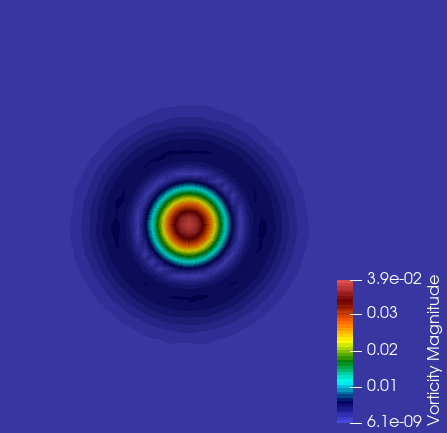
\includegraphics[width=\textwidth]{graphics/vorticityini.png}
         \caption{exact solution}
         \label{fig:3.1}
     \end{subfigure}
     \hspace{0.5cm}
     \begin{subfigure}[b]{0.35\textwidth}
         \centering
         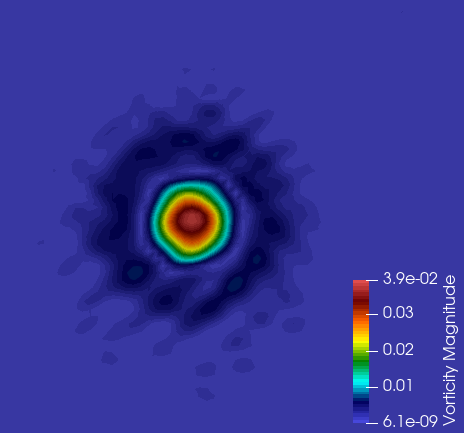
\includegraphics[width=\textwidth]{graphics/vorticityE2.png}
         \caption{with E2F10 scheme}
         \label{fig:3.1}
     \end{subfigure}

     \begin{subfigure}[b]{0.35\textwidth}
         \centering
         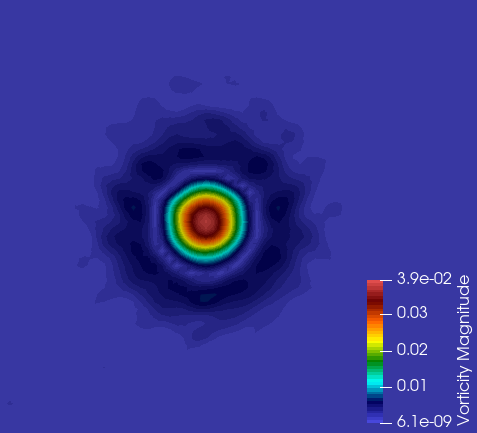
\includegraphics[width=\textwidth]{graphics/vorticityC4.png}
         \caption{with C4F10 scheme}
         \label{fig:3.1}
     \end{subfigure}
     \hspace{0.5cm}
     \begin{subfigure}[b]{0.35\textwidth}
         \centering
         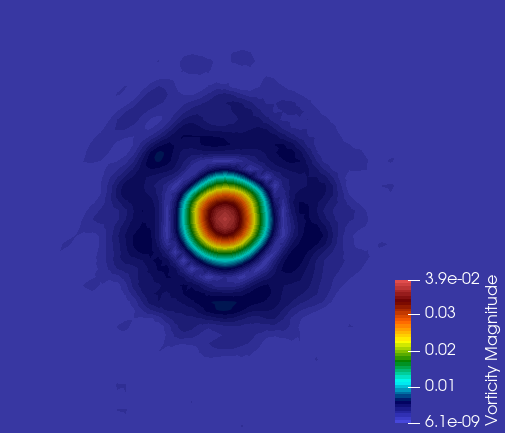
\includegraphics[width=\textwidth]{graphics/vorticityC6.png}
         \caption{with C6F10 scheme}
         \label{fig:3.1}
     \end{subfigure}
     \caption{Vorticity contours}
     \label{fig:3}
    \end{figure}

    \begin{figure}[h!]
        \centering
        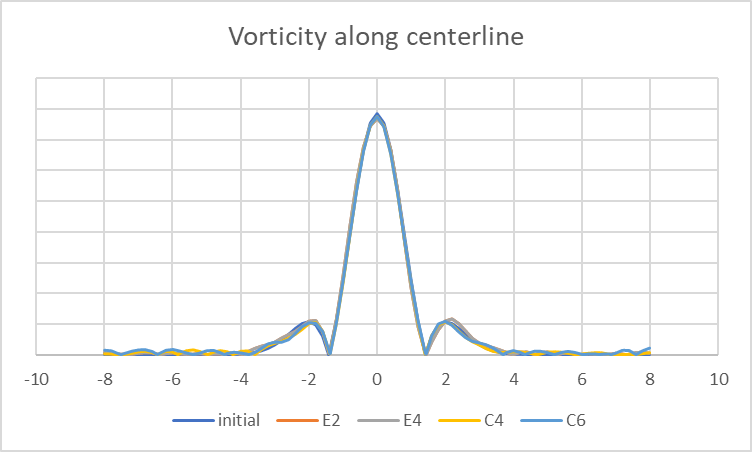
\includegraphics[width=0.5\linewidth]{graphics/center.png}
        \caption{Vorticity magnitude along center line for different schemes}
        \label{fig:my_label}
    \end{figure}

    All the schemes show noticeable variations from the exact solution (vortex at t$=0$). The errors are more prominent in the vortex boundaries. We can also see that compact schemes are much better at capturing the vortex then the explicit scheme.

    \subsection{Order of accuracy: }

    the following log-log plot was obtained for error analysis of all the 12 cases for E2, E4, C4 and C6 corresponding to $\frac{\Delta x}{R} =$ 0.2, 0.1, 0.05:
    
    \begin{figure}[h!]
        \centering
        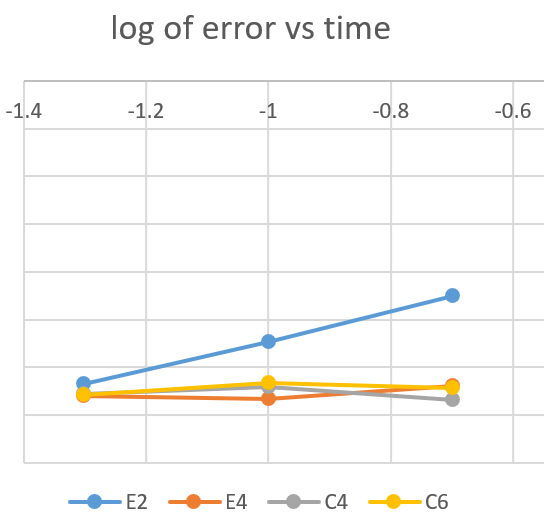
\includegraphics[width=0.5\linewidth]{graphics/error.png}
        \caption{log(error) v/s log($\Delta$x)}
        \label{fig:my_label}
    \end{figure}

    I did not get expected plots for the order of accuracy analysis. Only for E2 scheme, the slope came as expected = 1.7 ($\sim$ 2). I saved the v velocity from the initialized Qp arrays and tried to find the maximum difference between the initial and the final v velocity along the centerline (j=jmax/2). But I did not get desired results even after many corrections. This was a major cause of the delayed submission. 

    \subsection{Random grid: }

    \begin{figure}[H]
        \centering
        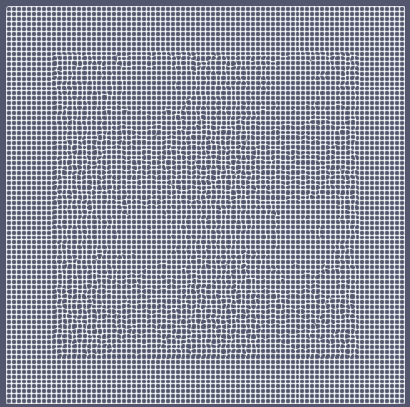
\includegraphics[width=0.4\linewidth]{graphics/Rgrid.png}
        \caption{Randomly perturbed mesh}
        \label{fig:my_label}
    \end{figure}

    \begin{figure}[H]
        \centering
        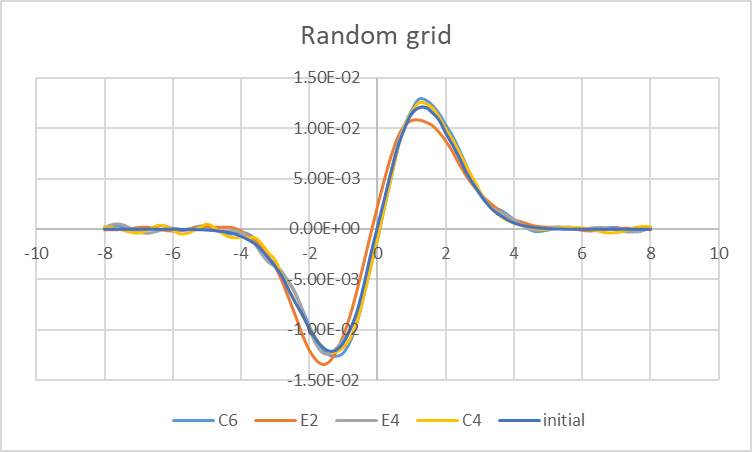
\includegraphics[width=0.6\linewidth]{graphics/random.png}
        \caption{v velocity along center line for different schemes in random mesh}
        \label{fig:my_label}
    \end{figure}

    We can see fluctuations in v velocity toward the boundaries. The same is also noticed in the vorticity plot, where oscillations in vorticity can be seen at the boundaries. E2 scheme gives the least accurate solution.

    \subsection{Sinous grid: }

    \begin{figure}[H]
        \centering
        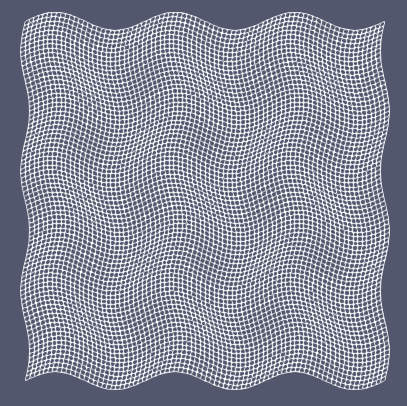
\includegraphics[width=0.4\linewidth]{graphics/Sgrid.png}
        \caption{Sinusoidal mesh}
        \label{fig:my_label}
    \end{figure}

    \begin{figure}[H]
        \centering
        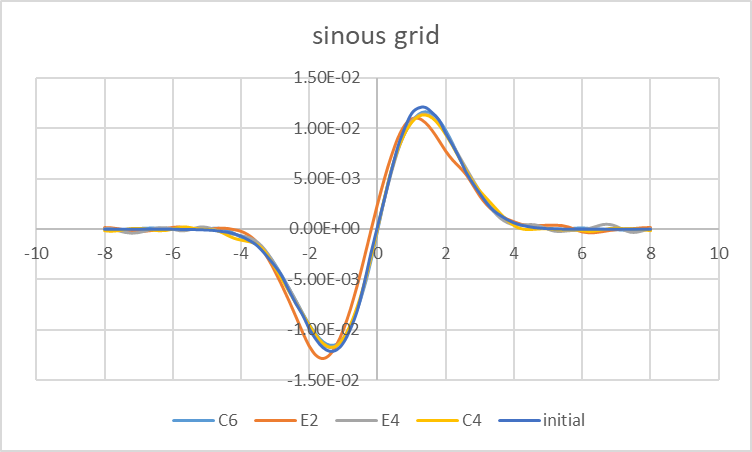
\includegraphics[width=0.6\linewidth]{graphics/sinous.png}
        \caption{v velocity along center line for different schemes in sinous}
        \label{fig:my_label}
    \end{figure}

    Similar trend as the random grid is obtained. Although the solution at the boundaries seems more stable than the random grid. We can also note that the solution to both sinusoidal and random grid is less accurate than that of uniform mesh.  
    
\end{document}
